\documentclass[11pt,a4paper]{article}
\usepackage{fontspec}
\setmainfont{texgyretermes}[Extension=.otf,UprightFont=*-regular,BoldFont=*-bold,ItalicFont=*-italic,BoldItalicFont=*-bolditalic]
\usepackage[margin=1.8cm,headheight=14pt]{geometry}
\usepackage{booktabs,longtable,array,ragged2e,enumitem,microtype,xcolor,graphicx,fancyhdr,amsmath}
\usepackage[hidelinks,unicode]{hyperref}
\definecolor{ink}{HTML}{193C49}\definecolor{teal}{HTML}{147D7B}\definecolor{pale}{HTML}{EAF4F2}
\newcolumntype{P}[1]{>{\RaggedRight\arraybackslash}p{#1}}
\setlength{\parindent}{0pt}\setlength{\parskip}{5pt}\setlength{\emergencystretch}{2em}
\setlength{\tabcolsep}{4pt}\renewcommand{\arraystretch}{1.14}
\setlist{nosep,leftmargin=1.3em,topsep=4pt}
\pagestyle{fancy}\fancyhf{}\fancyhead[L]{\small BẢO VỆ RIÊNG TƯ QUỸ ĐẠO}
\fancyhead[R]{\small Chuẩn bị 06/10/2026}\fancyfoot[C]{\small\thepage}
\renewcommand{\headrulewidth}{0.3pt}
\newcommand{\key}[1]{\par\smallskip\noindent\colorbox{pale}{\parbox{\dimexpr\linewidth-2\fboxsep}{\textbf{#1}}}\par\smallskip}
\begin{document}
\begin{center}{\LARGE\bfseries\color{ink}Bảo vệ riêng tư quỹ đạo với Geo-I}\\[5pt]{\large Kiến trúc, đối chứng và các cải tiến sau buổi gặp 03/10}\\[4pt]{\small Chuẩn bị 06/10/2026 · Buổi GVHD tiếp theo · Geo-I là nền tảng}\end{center}
\section*{1. Related works và cách so sánh công bằng}
Giữ Geo-I làm cơ chế bảo vệ GPS. Vòng này mở rộng dịch vụ POI, quản lý ngân sách qua nhiều chuyến và kiểm tra attacker kỹ hơn.

\begingroup\small
\begin{longtable}{@{}P{3.580cm}P{3.708cm}P{1.534cm}P{2.174cm}P{5.243cm}@{}}
\toprule
\textbf{Paper trong 3 năm} & \textbf{Output} & \textbf{Fully} & \textbf{Partially} & \textbf{Metrics gốc}\\\midrule
\endfirsthead
\toprule
\textbf{Paper trong 3 năm} & \textbf{Output} & \textbf{Fully} & \textbf{Partially} & \textbf{Metrics gốc}\\\midrule
\endhead\bottomrule\endfoot
\href{https://arxiv.org/html/2409.09495v1}{TransProtect (2024)} & Một vị trí nhiễu/mốc & S1, S3 & S2 & EIE $\uparrow$; chênh chi phí tới đích $\downarrow$; chưa khóa metric vận hành\\
\addlinespace[2pt]
\href{https://link.springer.com/article/10.1007/s44443-026-00899-w}{Semantic correlation (2026)} & GPS thật + dummy theo ngữ nghĩa/đường & S1 & S2, S3 & ASR $\uparrow$; DER $\uparrow$ (dummy hợp lý); thời gian tạo $\downarrow$\\
\addlinespace[2pt]
\href{https://link.springer.com/article/10.1007/s44443-025-00438-z}{Fake queries (2026)} & Tập thật + dummy, xen query giả & S1, S3 & S2 & ASR/số đường khó phân biệt $\uparrow$; thời gian/RSS $\downarrow$; chưa chấm POI\\
\addlinespace[2pt]
\href{https://uhra.herts.ac.uk/id/eprint/25705/}{CPCROK (2025)} & Beacon xe + tuyến giả, đổi pseudonym & — & S4 & Ghép đúng trace ρ $\downarrow$; số tuyến giả ψ $\downarrow$; chưa chấm POI\\
\addlinespace[2pt]
\href{https://www.aimspress.com/article/doi/10.3934/era.2025293}{DP-FETC (2025)} & Bộ trace tổng hợp offline & — & S3, S8, S9, S10 & MI $\downarrow$, $\varepsilon$-DP; JSD phân bố $\downarrow$; độ phức tạp\\
\addlinespace[2pt]
\href{https://wrap.warwick.ac.uk/id/eprint/183198/}{EV Geo-I querying (2024)} & AGeoI + dummy; Edge trộn query & — & S1, S2, S3 & ($\varepsilon$,δ)-AGeoI; CoP $\downarrow$, CoP=0 $\uparrow$; Wasserstein IBU $\downarrow$\\
\addlinespace[2pt]
\end{longtable}
\endgroup
Cửa sổ online đầu tiên: 06/10/2023–06/10/2026. \textbf{Fully:} trực tiếp xét và đánh giá task/threat trong giả định paper. \textbf{Partially:} cơ chế liên quan hoặc phạm vi hẹp hơn. Đây là đối chiếu của nhóm; scenario không ghi là chưa có bằng chứng trực tiếp. Geo-I (2013), DLS (2014), RDG (2021) là nền tảng ngoài cửa sổ.

S1 vị trí; S2 nơi dừng; S3 đoạn đường; S4 liên kết danh tính người/xe; S5 đường kế tiếp; S6 đích tương lai; S7 ý định query; S8 dữ liệu người đi cùng; S9 điểm đầu bị che; S10 điểm cuối của chuyến đã kết thúc.

\begin{itemize}
\item \textbf{Output khác nhau:} một vị trí, tập thật + dummy, Q-only hoặc dataset offline; ASR cần thành viên thật nên không áp trực tiếp cho Q-only.
\item \textbf{Metrics trả lời khác câu hỏi:} entropy/DER đo độ khó phân biệt hoặc tính hợp lý; $\varepsilon$ đo giới hạn cơ chế; chúng chưa đo đồng thời khả năng attacker và chất lượng POI.
\item \textbf{Dùng hai lớp đo:} Hit100/MAE + Recall@5 + chi phí trên cùng protocol; thêm metrics gốc khi đúng output và đủ dữ liệu. N/A phải có lý do.
\end{itemize}
\clearpage
\section*{2. Kiến trúc: từ GPS tới câu trả lời POI}
\begin{center}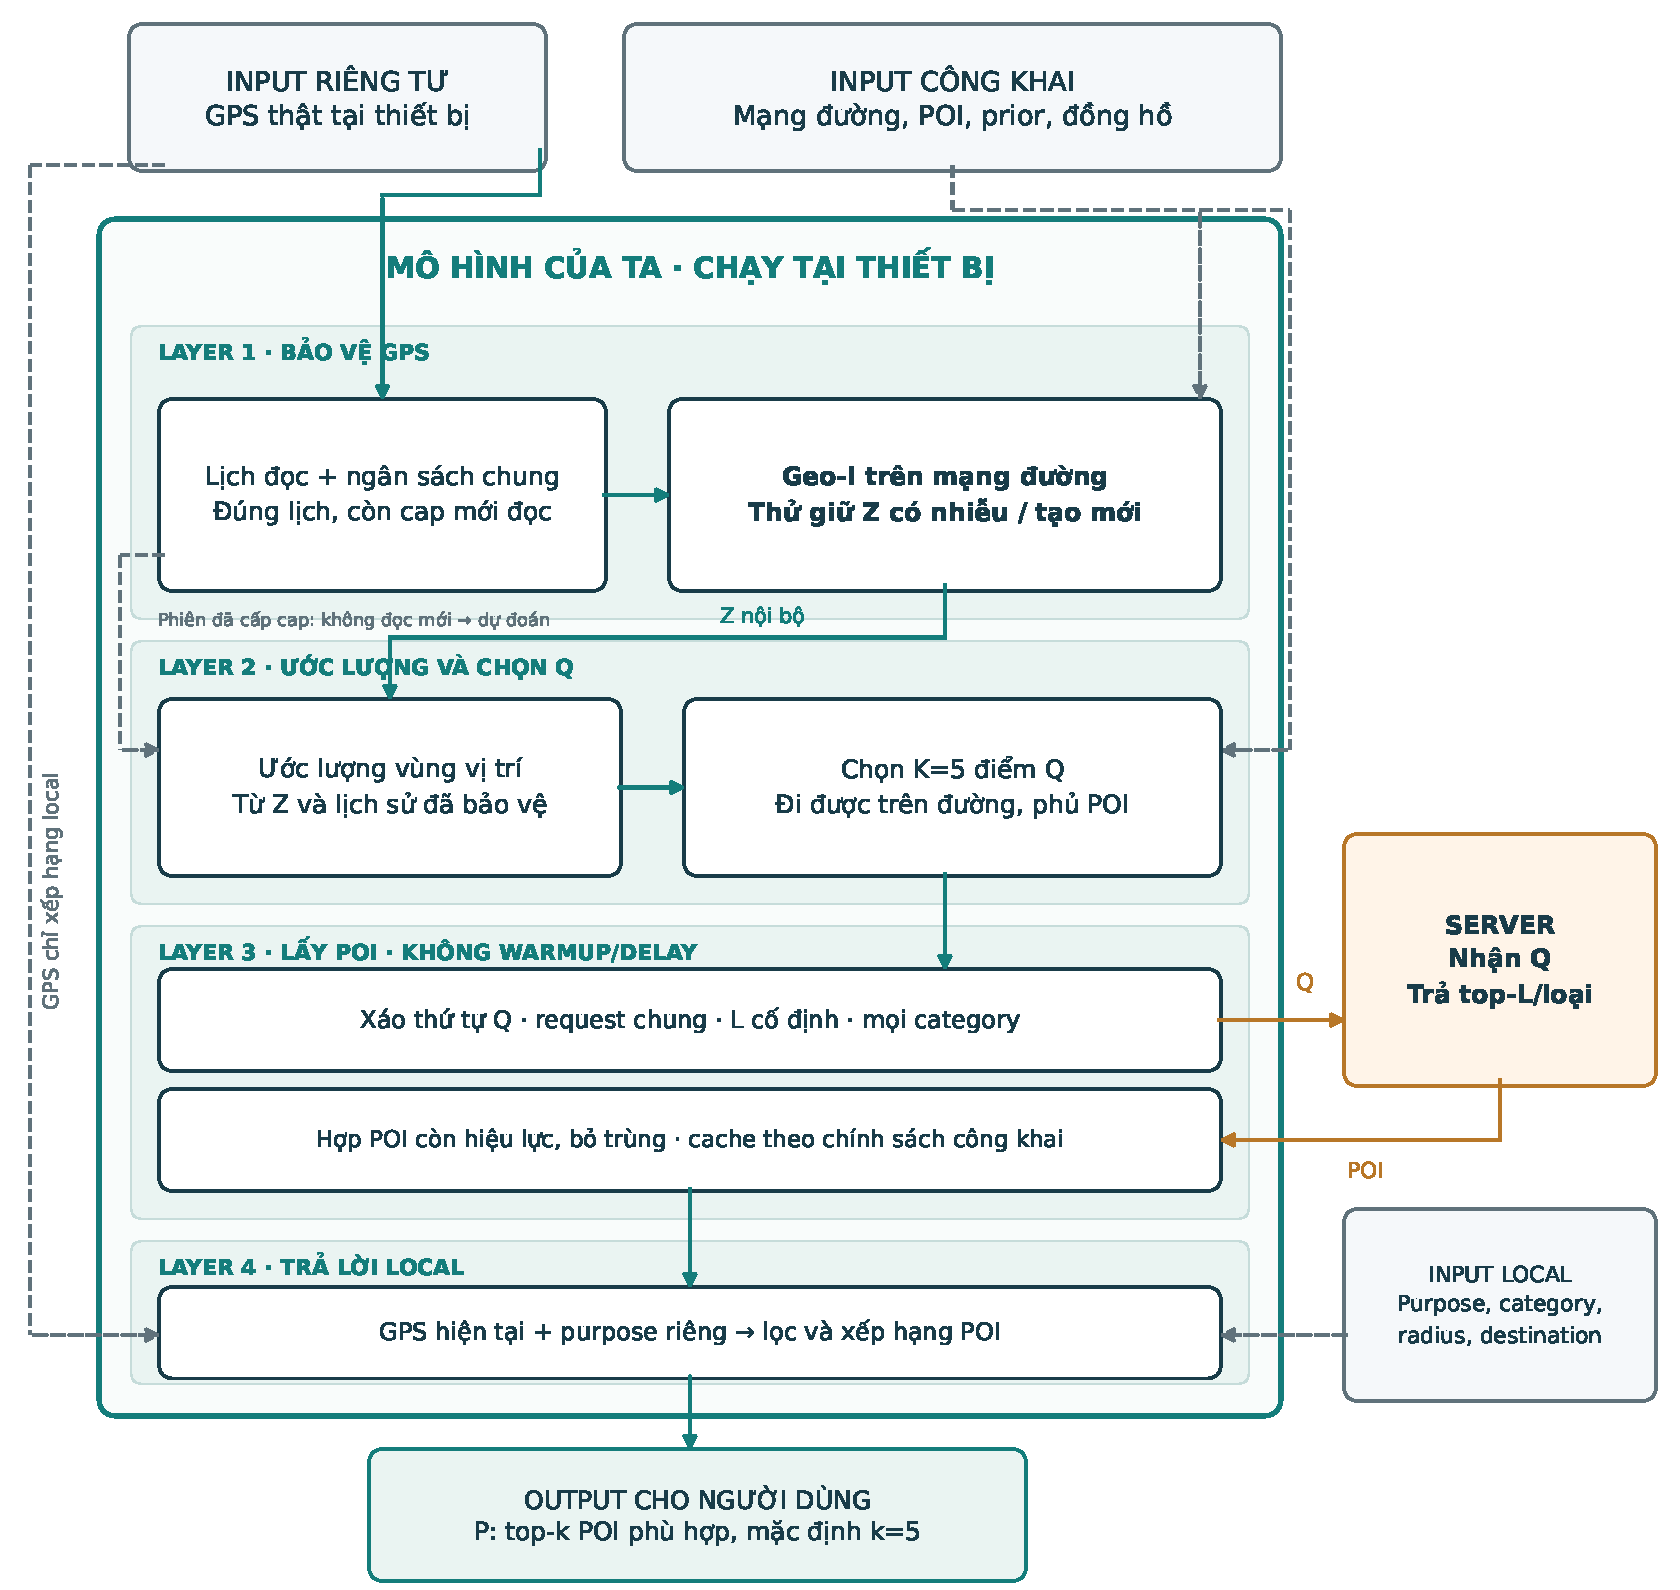
\includegraphics[width=\linewidth,height=18.5cm,keepaspectratio]{figures/architecture.pdf}\end{center}
{\small Mũi tên liền: luồng xử lý. Nét đứt: input/phương án không đọc GPS mới. \textbf{Z} nội bộ; \textbf{Q} gửi server; \textbf{P} là POI trả cho người dùng.}
\textbf{Layer 2} cập nhật vùng vị trí có thể xảy ra từ Z, lịch sử đã bảo vệ và khả năng di chuyển trên đường. Nó giúp chọn Q khả thi, phủ POI tốt; phiên đã cấp cap vẫn có thể dự đoán khi không đọc GPS mới. Phiên vượt giới hạn chung không đọc GPS, không gửi Q. Purpose thật chỉ dùng ở layer 4.

\textbf{S1–S3:} Geo-I và phép thử tái dùng Z có nhiễu. \textbf{S9/S10:} nhiễu mạnh hơn ở mọi lần đọc, vì online chưa biết lần nào là cuối. \textbf{S7:} request chung, lọc purpose locally. \textbf{S4–S6:} ngân sách chung hạn chế tích lũy, chưa tự giấu danh tính. S8 chưa có đánh giá mới.

\clearpage
\section*{3. Cấu hình và attacker trước khi đọc kết quả}
\begingroup\small
\begin{longtable}{@{}P{4.661cm}P{6.080cm}P{6.080cm}@{}}
\toprule
\textbf{Tham số} & \textbf{GeoI-Endpoint20} & \textbf{GeoI-Epoch8-H12}\\\midrule
\endfirsthead
\toprule
\textbf{Tham số} & \textbf{GeoI-Endpoint20} & \textbf{GeoI-Epoch8-H12}\\\midrule
\endhead\bottomrule\endfoot
Mục tiêu & Kiểm tra S9/S10 không delay & S5/S6 và utility qua 8 chuyến\\
\addlinespace[2pt]
$\varepsilon$ thử = $\varepsilon$ tạo Z, đơn vị /m & 0,0025 & 0,00125\\
\addlinespace[2pt]
H: số lần đọc tối đa/chuyến & 12 & 12\\
\addlinespace[2pt]
B: ngân sách danh nghĩa/chuyến & 0,06 & 0,03\\
\addlinespace[2pt]
Cap hiệu dụng/chuyến & 0,0575 & 0,02875\\
\addlinespace[2pt]
Ngân sách qua nhiều chuyến & Cộng theo số chuyến; chưa là cap chung & N=8; tổng C=0,23/m\\
\addlinespace[2pt]
Lịch, điểm Q và kết quả & GPS 60s; K=5; L=20; k=5 & GPS 60s; K=5; L20 chọn bằng utility\\
\addlinespace[2pt]
Đồng hồ gửi Q công khai & Mỗi 60s trong cohort endpoint & Mỗi 20s + mốc hiệu chuẩn công khai\\
\addlinespace[2pt]
Quy tắc khác & Ngưỡng 200m; slack 0,03 & Cùng backbone; cache local riêng\\
\addlinespace[2pt]
Warmup / delay & 0 / 0 & 0 / 0\\
\addlinespace[2pt]
\end{longtable}
\endgroup
Đây là các cấu hình của cùng thuật toán. Với cap chung C, tối đa N chuyến và horizon H công khai: \textbf{u=C/[N(2H−1)]}, $\varepsilon$ thử=$\varepsilon$ tạo=u, B=2Hu. H/N được đặt trước; giữ phần cap trong sổ trước GPS; không cấp lại khi restart. K là số Q, L là số POI/loại mỗi Q, k là số câu trả lời tối đa.

\begin{itemize}
\item \textbf{S1–S3, bảng đối chứng:} \textbf{Shadow KNN (k=3)} cùng centroid, continuity, road filter và decoder đường. S2 thêm running mean/intersection khi output chứa GPS thật.
\item \textbf{S7:} \textbf{kNN, ExtraTrees, logistic} đoán purpose/category từ request, reply, tọa độ, thời gian và kích thước.
\item \textbf{S4:} \textbf{kNN/ExtraTrees} liên kết cặp phiên từ summary/shape; \textbf{S5/S6:} \textbf{ExtraTrees trên hình học ứng viên}, decoder đường/lịch sử và uniform.
\item \textbf{S9/S10 mới:} \textbf{OLS, kNN, ExtraTrees, Viterbi}, gồm tracking \textbf{Hungarian}. Chọn riêng cho MAE/Hit trên validation; khóa trước chấm test.
\end{itemize}
\key{Hit100 $\downarrow$: tỷ lệ đoán trong 100m. MAE $\uparrow$: sai số attacker trung bình (m). Recall@5 $\uparrow$: phần POI chuẩn tìm lại được. Ở S1, 33,33\% / 299m nghĩa attacker đúng trong 100m ở 1/3 số mốc, sai trung bình 299m.}
Lúc chấm test, attacker chỉ thấy dữ liệu công bố và thông tin phụ đã định; GPS/nhãn test thuộc evaluator. GPS/nhãn shadow-train được phép dùng để học attacker. Raw kiểm tra bài toán có tín hiệu. Các họ attacker áp cho mọi phương pháp phù hợp, học/chọn riêng theo output; không chỉ có một Shadow KNN.

\clearpage
\section*{4. Đối chứng trên cùng protocol và metrics gốc}
Bảng paper-v2 giữ nguyên: 12 chuyến test, cùng trace/dịch vụ/split và họ attacker. \textbf{Dấu * là adaptation tại repo}, chưa tái lập đầy đủ paper. Mỗi ô là \textbf{Hit100 / MAE(m) / Recall@5}, gộp đều theo chuyến; các phương pháp không cùng bảo đảm $\varepsilon$.

\begingroup\small
\begin{longtable}{@{}P{3.489cm}P{2.492cm}P{2.492cm}P{2.492cm}P{2.492cm}P{2.492cm}@{}}
\toprule
\textbf{Phương pháp} & \textbf{S1} & \textbf{S2} & \textbf{S3} & \textbf{S9} & \textbf{S10}\\\midrule
\endfirsthead
\toprule
\textbf{Phương pháp} & \textbf{S1} & \textbf{S2} & \textbf{S3} & \textbf{S9} & \textbf{S10}\\\midrule
\endhead\bottomrule\endfoot
GPS thật & 100,00\% / 13 / 100,00\% & 100,00\% / 39 / 100,00\% & 96,43\% / 23 / 100,00\% & 41,67\% / 120 / 100,00\% & 8,33\% / 630 / 100,00\%\\
\addlinespace[2pt]
DLS* & 58,33\% / 1.318 / 100,00\% & 100,00\% / 39 / 100,00\% & 31,21\% / 1.688 / 100,00\% & 8,33\% / 1.582 / 100,00\% & 0,00\% / 2.029 / 100,00\%\\
\addlinespace[2pt]
TransProtect* & 83,33\% / 84 / 97,78\% & 66,67\% / 88 / 97,19\% & 69,28\% / 99 / 97,93\% & 25,00\% / 184 / 97,27\% & 8,33\% / 680 / 98,52\%\\
\addlinespace[2pt]
Semantic* & 100,00\% / 11 / 100,00\% & 100,00\% / 42 / 100,00\% & 40,58\% / 257 / 100,00\% & 33,33\% / 132 / 100,00\% & 16,67\% / 731 / 100,00\%\\
\addlinespace[2pt]
\textbf{BR-Dummy / Geo-I} & \textbf{33,33\% / 299 / 95,83\%} & \textbf{22,22\% / 247 / 97,01\%} & \textbf{7,44\% / 776 / 87,67\%} & \textbf{0,00\% / 316 / 96,60\%} & \textbf{0,00\% / 2.315 / 88,33\%}\\
\addlinespace[2pt]
\end{longtable}
\endgroup
BR có Hit100 thấp hơn hoặc bằng ba adaptations ở cả năm scenario. MAE lớn hơn TransProtect ở cả năm; DLS có MAE lớn hơn BR ở S1/S3/S9. Recall S3/S10 của BR dưới 90\%. \textbf{Chưa thể nói thắng mọi metric.} Raw S9/S10 chỉ thấy cửa sổ sau che đầu/cuối; sai số còn bao gồm độ khó của masking.

\begingroup\small
\begin{longtable}{@{}P{4.959cm}P{3.306cm}P{4.132cm}P{4.132cm}@{}}
\toprule
\textbf{Phương pháp} & \textbf{Recall macro $\uparrow$} & \textbf{JSON bytes/mốc $\downarrow$} & \textbf{Tạo output ms/mốc $\downarrow$}\\\midrule
\endfirsthead
\toprule
\textbf{Phương pháp} & \textbf{Recall macro $\uparrow$} & \textbf{JSON bytes/mốc $\downarrow$} & \textbf{Tạo output ms/mốc $\downarrow$}\\\midrule
\endhead\bottomrule\endfoot
GPS thật & 100,00\% & 720 & 0,01\\
\addlinespace[2pt]
DLS* & 100,00\% & 3.282 & 1,01\\
\addlinespace[2pt]
TransProtect* & 97,74\% & 720 & 0,35\\
\addlinespace[2pt]
Semantic* & 100,00\% & 3.287 & 1,17\\
\addlinespace[2pt]
\textbf{BR-Dummy / Geo-I} & 93,09\% & 3.237 & 5,40\\
\addlinespace[2pt]
\end{longtable}
\endgroup
\begin{itemize}
\item \textbf{EIE point estimate:} có thể tính lại; cùng ước lượng/khoảng cách/phép gộp thì đúng bằng MAE ở trên, không là bằng chứng thứ hai.
\item \textbf{ASR/entropy/DER:} N/A khi thiếu posterior/prior hoặc quy tắc dummy gốc. Q-only không có vị trí thật làm thành viên để chấm ASR.
\item \textbf{Δc của TransProtect:} N/A trong archive cũ vì thiếu cost tables/prior đích gốc. Diagnostic riêng trên mạng đường: Raw 0m, Endpoint20 trung bình Q 1.386,74m; đây là méo chi phí $\downarrow$, không phải privacy và không là head-to-head paper.
\end{itemize}
Chi phí bảng này gồm request JSON + response ID POI, chưa HTTP/TLS; thời gian trên máy benchmark cũ. Các thử nghiệm sau dùng cohort/protocol khác và được đọc riêng. \href{evidence.json}{Nguồn và định nghĩa}.

\clearpage
\section*{5. S7: nhiều purpose, cùng request ra mạng}
Mọi Q lấy POI của các loại theo L cố định. Thiết bị hợp và bỏ trùng; sau đó GPS thật + purpose riêng tư quyết định câu trả lời. Đổi purpose/category/radius/destination không đổi Q, request hoặc lịch gửi.

\begingroup\small
\begin{longtable}{@{}P{11.407cm}P{5.703cm}@{}}
\toprule
\textbf{Purpose đã hiện thực} & \textbf{Recall@5, cấu hình giữ lại}\\\midrule
\endfirsthead
\toprule
\textbf{Purpose đã hiện thực} & \textbf{Recall@5, cấu hình giữ lại}\\\midrule
\endhead\bottomrule\endfoot
Gần nhất theo quãng đường & 96,33\%\\
\addlinespace[2pt]
Đến nhanh nhất & 96,33\%\\
\addlinespace[2pt]
Trong bán kính riêng tư & 90,10\%\\
\addlinespace[2pt]
Ít vòng đường tới đích riêng tư & 94,57\%\\
\addlinespace[2pt]
\end{longtable}
\endgroup
Cohort development 3 nhóm, 2 RNG/chuyến; giữ $\alpha$=0,L20 vì các mục tiêu Q mới chưa đạt đồng thời yêu cầu privacy/byte. Mean bốn purpose \textbf{94,33\%}, không trả POI vi phạm điều kiện. Mạng này có tốc độ đồng nhất nên gần nhất/nhanh nhất trùng ranking; kiểm thử với tốc độ khác xác nhận hai hàm khác nhau.

Audit nội dung: payload tường minh bị đoán purpose 100\%; request chung 25\% cho bốn purpose, 16,67\% cho sáu category. Đây là kiểm tra kênh nội dung trực tiếp; tuyến đường đặc trưng, account hoặc click vẫn có thể tiết lộ nhu cầu. Giá/giờ mở cửa/trạng thái realtime cần metadata riêng.

\subsection*{Cải thiện utility mà giữ nguyên Q và Geo-I}
\begingroup\small
\begin{longtable}{@{}P{6.358cm}P{3.179cm}P{3.179cm}P{3.815cm}@{}}
\toprule
\textbf{GeoI-Epoch8-H12, cohort native} & \textbf{Recall toàn cửa sổ} & \textbf{Recall 400–600s} & \textbf{Chuyến thấp nhất, 400–600s}\\\midrule
\endfirsthead
\toprule
\textbf{GeoI-Epoch8-H12, cohort native} & \textbf{Recall toàn cửa sổ} & \textbf{Recall 400–600s} & \textbf{Chuyến thấp nhất, 400–600s}\\\midrule
\endhead\bottomrule\endfoot
L10, phản hồi hiện tại & 89,95\% & 90,29\% & 66,36\%\\
\addlinespace[2pt]
L20, phản hồi hiện tại & 94,96\% & 94,39\% & 70,30\%\\
\addlinespace[2pt]
L20, cache 60s & 95,64\% & 95,22\% & 72,42\%\\
\addlinespace[2pt]
\textbf{L20, cache POI cố định theo phiên bản} & 99,34\% & 99,48\% & 86,67\%\\
\addlinespace[2pt]
\end{longtable}
\endgroup
Sáu nhóm test, 8 chuyến/nhóm. Cache mới chỉ giữ \textbf{metadata POI cố định đã nhận trước đó}, dùng qua các chuyến trong cùng epoch công khai; hết epoch/đổi phiên bản thì vô hiệu. Không đọc dữ liệu tương lai, không tải thêm POI theo nhu cầu. Tối đa 416/418 ID trong test.

Ba phương án L20 cùng \textbf{7.550 request Q, 41.233.562 reply JSON bytes}; L20 tốn khoảng 1,56$\times$ reply L10. Recall là conditional: 1.402/1.510 mốc có reference (92,85\%); đoạn cuối 462/528 (87,50\%). Chuyến đầu chưa có cache còn yếu. Trạng thái đang mở/còn chỗ phải có dữ liệu mới, nếu thiếu là chưa biết.

Cache đã có adapter client tùy chọn và replay causal trên transcript đóng băng; client mặc định vẫn cache epoch60. Đây là xử lý local dùng được cho cả đối chứng: reset từng chuyến cùng cache đạt 99,82\%. Không thay bảng privacy S5/S6; cần confirmation độc lập sau vòng development này.

\clearpage
\section*{6. S4–S6: ngân sách chung và suy tương lai}
\begingroup\small
\begin{longtable}{@{}P{6.315cm}P{2.786cm}P{4.086cm}P{3.343cm}@{}}
\toprule
\textbf{S4, cohort development} & \textbf{Cap /6 chuyến} & \textbf{AUC người / xe} & \textbf{Recall@5 $\uparrow$}\\\midrule
\endfirsthead
\toprule
\textbf{S4, cohort development} & \textbf{Cap /6 chuyến} & \textbf{AUC người / xe} & \textbf{Recall@5 $\uparrow$}\\\midrule
\endhead\bottomrule\endfoot
GPS thật & — & 0,773 / 0,716 & 100,00\%\\
\addlinespace[2pt]
Geo-I reset từng chuyến & 0,345 & 0,632 / 0,544 & 97,03\%\\
\addlinespace[2pt]
GeoI-Epoch6-H12 & 0,23 & 0,640 / 0,577 & 95,53\%\\
\addlinespace[2pt]
\textbf{GeoI-Epoch6-H8} & 0,23 & 0,526 / 0,504 & 97,23\%\\
\addlinespace[2pt]
\end{longtable}
\endgroup
AUC gần 0,5 nghĩa attacker đã chọn chưa phân biệt ổn định trong mẫu này. H8 chỉ có 3 nhóm test đã dùng trong phát triển; audit bank có raw AUC theo nhóm tới 0,694 và 0,229 (đảo chiều), nên chưa kết luận khó liên kết. H12 chưa tốt hơn reset. \textbf{Ở cùng tổng cap, đổi cách ghi sổ không đổi output hoặc điểm attacker.} Sổ giúp thực thi cap qua nhiều phiên, chưa che account/IP/biển số.

\subsection*{S5/S6 trên prefix thật của native SUMO}
\begingroup\small
\begin{longtable}{@{}P{6.199cm}P{3.444cm}P{3.444cm}P{3.444cm}@{}}
\toprule
\textbf{Sau khi bắt đầu rẽ} & \textbf{S5 đúng cạnh $\downarrow$} & \textbf{S6 Hit100 $\downarrow$} & \textbf{S6 MAE(m) $\uparrow$}\\\midrule
\endfirsthead
\toprule
\textbf{Sau khi bắt đầu rẽ} & \textbf{S5 đúng cạnh $\downarrow$} & \textbf{S6 Hit100 $\downarrow$} & \textbf{S6 MAE(m) $\uparrow$}\\\midrule
\endhead\bottomrule\endfoot
GPS thật & 100,00\% & 100,00\% & 5\\
\addlinespace[2pt]
Geo-I reset từng chuyến & 41,67\% & 41,67\% & 661\\
\addlinespace[2pt]
\textbf{GeoI-Epoch8-H12} & 50,00\% & 50,00\% & 543\\
\addlinespace[2pt]
\end{longtable}
\endgroup
24 nhóm, 192 chuyến; 12 train/6 chọn/6 test. Attacker biết hai hướng rẽ/đích có thể xảy ra và sáu lịch sử đã bảo vệ; chỉ thấy prefix tới mốc công khai. Các cạnh test chưa xuất hiện trong train. Sau rẽ Raw 100\% xác nhận có tín hiệu; trước rẽ Raw cũng 50\%, là mơ hồ có sẵn.

Epoch8 giữ tổng cap 0,23/m cho tám chuyến, reset có tổng 1,84/m. Epoch8 chọn uniform trên selection và chưa tốt hơn reset về attacker; hai target cùng dựa trên một lựa chọn hướng rẽ nên không là hai bằng chứng độc lập. Attacker chưa dùng đầy đủ các liên kết giữa tám chuyến.

\key{Đóng góp đã có: cap không cấp lại theo chuyến/restart; prefix tương lai được chấm đúng thời điểm; utility phục hồi bằng L/cache local. Chưa chứng minh giấu toàn bộ danh tính hoặc thắng mọi dự báo tương lai.}
\clearpage
\section*{7. S9/S10: nhiễu không delay và kiểm tra attacker}
Không bỏ đoạn đầu và không trì hoãn đoạn cuối. Endpoint20 dùng $\varepsilon$ nhỏ hơn trên \textbf{mọi lần đọc} vì chưa biết trước đâu là lần cuối. So với GeoI-Slack20: cùng backbone, K=5/L20, mọi mốc được gửi; $\varepsilon$ giảm 0,01 $\rightarrow$ 0,0025/m.

\begingroup\small
\begin{longtable}{@{}P{5.515cm}P{2.605cm}P{2.605cm}P{2.758cm}P{2.758cm}@{}}
\toprule
\textbf{28 nhóm, 112 runs/phương pháp} & \textbf{S9 MAE$\uparrow$} & \textbf{S10 MAE$\uparrow$} & \textbf{S10 Hit100$\downarrow$} & \textbf{S10 Hit500$\downarrow$}\\\midrule
\endfirsthead
\toprule
\textbf{28 nhóm, 112 runs/phương pháp} & \textbf{S9 MAE$\uparrow$} & \textbf{S10 MAE$\uparrow$} & \textbf{S10 Hit100$\downarrow$} & \textbf{S10 Hit500$\downarrow$}\\\midrule
\endhead\bottomrule\endfoot
GeoI-Slack20 (đối chứng cùng L) & 790 & 758 & 0,00\% & 12,50\%\\
\addlinespace[2pt]
\textbf{GeoI-Endpoint20} & 1.407 & 1.337 & 0,00\% & 4,46\%\\
\addlinespace[2pt]
\end{longtable}
\endgroup
Chọn attacker bằng cross-fit theo nhóm: lần lượt giữ ngoài 1 trong 8 nhóm train, cộng 2 nhóm selection; ưu tiên điểm ổn định hơn qua nhóm, không chọn bằng test. Attacker GeoI-Slack20 có MAE S10 \textbf{758m} thay vì 901m ở bank cũ; Endpoint20 vẫn \textbf{1.337m}. Chênh MAE cùng L: \textbf{579 m; khoảng bootstrap 95\% [468; 696] m}. Bootstrap theo nhóm, không coi 112 runs là độc lập.

Hit100 đều 0\% nên không phân biệt hai cấu hình; thêm Hit500 cho thước đo rộng hơn. Quy tắc mới cải thiện MAE nhưng Hit chưa ổn định: trên Slack L10, Hit500 S10 giảm 30,36\% $\rightarrow$ 14,29\%. Không gọi attacker mới tốt hơn ở mọi metric.

Endpoint20 Recall \textbf{96,64\%} ở cohort này, giảm khoảng 2,30 điểm \% so với Slack20; 6/112 runs dưới 90\%, thấp nhất 77,61\%. Xáo thứ tự Q bỏ nhãn slot nhưng Hungarian vẫn ghép được bằng hình học; không xem shuffle là lợi thế privacy độc lập.

\subsection*{Bước tiếp theo để kết luận chắc hơn}
\begin{itemize}
\item Khóa policy/cache/selector, chạy nhóm và thành phố chưa dùng để chỉnh phương pháp; ưu tiên chuyến đầu và chuyến dài có Recall thấp.
\item Mở rộng attacker liên kết toàn bộ lịch sử S4–S6; kiểm tra category/purpose lệch tần suất và suy ý định từ tuyến đường.
\item Bổ sung metadata và metrics gốc đúng hợp đồng từng paper; báo cả privacy, utility, chi phí và N/A. Giữ Geo-I làm nền tảng.
\end{itemize}
Các vòng mới là development/diagnostic, chưa là confirmation chưa từng xem. Kernel Geo-I lý tưởng là nền tảng; sampler float hiện tại vẫn xấp xỉ. S8 và các kênh account/IP chưa được giải quyết. \href{../../../artifacts/benchmarks/endpoint\_robust\_selection\_20261006/readout.json}{Endpoint evidence} · \href{../../../artifacts/benchmarks/native\_versioned\_static\_20261006\_v1/results.json}{Cache evidence}.

\end{document}
